\section{Concepts clés du sujet}

\subsection{Vocabulaire}

La compréhension de certains concepts est indispensable à la compréhension du 
sujet.

\subsubsection{Dossier de Transfert}

Un dossier de transfert est l'ensemble des documents fournis par un client 
dans le but de l'exécution d'une opération à l'étranger. Ces documents sont de 
plusieurs types et sont principalement composés de:

\begin{description}
  \item{\textbf{Un ordre de virement :}} Il est donné par le propriétaire d'un compte
    bancaire qui doit payer une prestation ou un créancier ou faire un 
    transfert. L'ordre de virement demande à la banque de débiter une somme de 
    son compte pour créditer un autre compte. Le compte à créditer peut se 
    trouver dans la même banque ou dans une autre banque. Ce document est
    obligatoire dans la réalisation d'une opération
   
  \item{\textbf{Une autorisation de change :}} Il s'agit d'un document obligatoire dans 
  la constitution d'un dossier de transfert à l'étranger. Ces opérations
    s'effectuant en dévise, l'autorisation de change autorise le change vers la
    dévise dans laquelle le transfert sera effectué.
    
  \item{\textbf{La délaration préalable d'importation :}} La Déclaration Préalable 
    d’Importation (DPI) est une formalité accomplie  au sein du ministère en 
    charge du commerce préalablement à toute opération d’importation de 
    marchandises dont la valeur FOB est supérieure ou égale à 500 000 FCFA.
    
  \item{\textbf{L'autorisation spéciale d'importation ou d'exportation :}} Ces documents 
    concernent des produits dont la liste est fixée par avis ministériel. De ces 
    produits, nous pouvons citer le sésame, les céréales, les amande de Karité,
    le sucre\ldots
 
  \item{\textbf{Les documents justifiant l'opération :}} Il s'agit pour des achats de
    marchandise des factures par exemple, pour une inscription dans une école de
    l'attestation d'inscription et du passeport du concerné, pour le règlement 
    d'un salaire du contrat de travail et du bulletin de paie \ldots. 
\end{description} 
   
   Les documents entrants en compte dans la constitution d'un dossier sont 
   nombreux et les éléments cités ci-dessus sont loin d'être exhaustifs.  

L'analyse d'une opération à l'étranger revient à analyser l'ensemble des 
informations contenues sur chacun de ces documents.

\subsubsection{Pays étranger}

Le terme étranger désigne tous les pays en dehors de l’UEMOA. Les 
transferts dans ces pays s'effectue en dévise.

Selon la terminologie du règlement 09/2010/CM/UEMOA relatif aux relations 
financières extérieurs des états membres de l'UEMOA, 
\begin{quote}
 \textit{Le terme étranger désigne  tous les pays en dehors de l'UEMOA pour le 
 contrôle de la position des établissements de crédit vis-à-vis de 
 l'étranger aainsi que pour le traitement des opérations suivantes: 
 domiciliation des exportations sur l'étranger et rapatriement du produit 
 de leur recettes, émission et mise en vente de valeurs mobilières 
 étrangères, importation et exportation d'or, opération d'investissement
 et d'emprunt avec l'étranger, exportation matérielle des moyens de 
 paiement et de valeurs mobilières par colis postaux ou envois par la 
 poste.}
\end{quote}

\subsubsection{Résidents et Non-Résidents dans un Etat}

Sont considérés comme résidents les personnes physiques ayant leur résidence
habituelle dans l'Etat considéré. Sont considérés comme non-résidents ayant leur
résidence habituelles à l'étranger.


Les opérations à l'étranger sont nombreuses et pour chaque type d'opération, les 
intervenants ou acteurs de la transaction sont différents.

\subsection{ Les diférentes opérations à l'étranger}

Plusieurs types d'opérations sont effectuées par le service des opérations 
internationales de la SGBF.

\subsubsection{Les transferts émis}

Il s'agit d'opérations émises  par la banque résidente en l'occurence la SGBF
à destination d'une autre banque présente dans un autre pays. On distingue 
quatres intervenants dans une opération de transfert émis:
\begin{itemize}
  \item L'émetteur de l'ordre qui est le donneur d'ordre
  \item La banque domiciliatrice de l'émetteur en l'occurence dans notre cas la
    SGBF.
  \item La banque du bénéficiaire de l'ordre
  \item Le Bénéficiaire de l'ordre
\end{itemize}

Dans le cas de la SGBF et de toutes les filiales SG, il existe des hubs en 
l'occurance SG New York pour les opérations en dollars et SG Paris pour toute 
les autres dévises. Les différents ordres sont envoyés vers ces hubs qui sont 
chargés de les acheminer vers les différentes banques bénéficiaires.   

 \subsubsection{Les transferts reçus}
   Par transfert reçu, on entend tout virement en provenance de l'étranger à
   destination d'une banque résidente. Les transferts reçus s'effectue par 
   transmission à la banque réceptrice d'un message SWIFT. Comme dans le cas des
   transferts émis nous distinguons quatres intervenants dans cette opération.
   
 \subsubsection{Les opérations de crédit documentaire}
   Le Crédit Documentaire est l’opération par laquelle une banque s’engage, à la
   demande et pour le compte de son client importateur, à régler à un tiers 
   exportateur, dans un délai déterminé, un certain montant contre remise des 
   documents strictement conformes et cohérents entre eux, justifiant de la 
   valeur et de l’expédition des marchandises ou des prestations de services.
   On distingue quatre intervenants pour assurer la sécurité de l'opération:
   \begin{itemize}
     \item L'Acheteur/Importateur = Donneur d'ordre
     \item La Banque de l'Acheteur = Banque Emettrice
     \item La Banque du vendeur = Banque notificatrice et/ou Banque confirmatrice
     \item Le vendeur/L'Exportateur = Bénéficiaire
   \end{itemize}
   \begin{figure}[h!]
     \begin{center}
       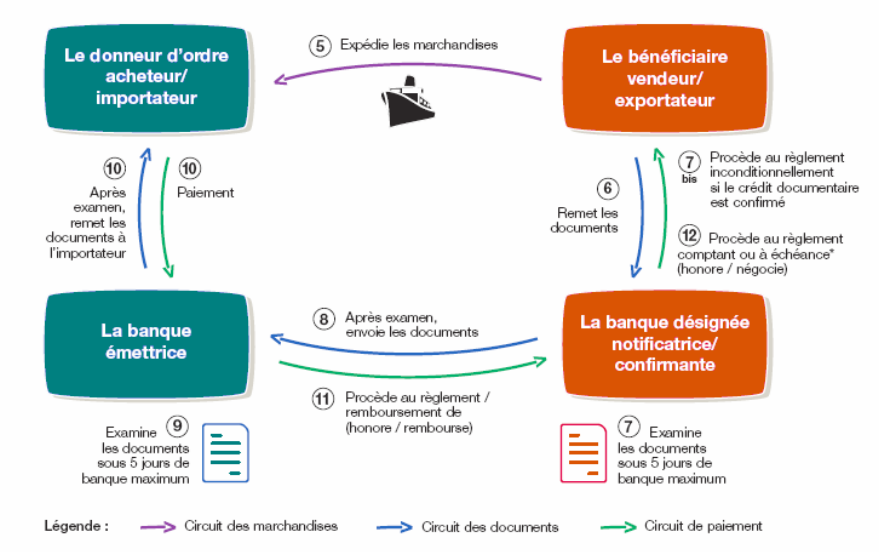
\includegraphics[width=12cm]{images/credit_doc.png}
        \caption{Circuit d'une opération de crédit documentaire.
        \label{fig:credit}}
     \end{center}
   \end{figure}
   
 \subsubsection{Les opérations de remise documentaire}
 
  La remise documentaire consiste pour le vendeur à faire encaisser par une 
  banque le montant dû par un acheteur contre remise de documents. Les
  documents sont remis à l'acheteur uniquement contre paiement ou acceptation
  d'une lettre de change.
  Les intervenants dans l'opération d'encaissement sont :
  \begin{itemize}
    \item Le Donneur d'ordre (le client)
    \item La Banque remettante (la banque du client)
    \item La banque chargée de l'encaissement (autre banque que la banque remettante)
    \item La Banque présentatrice (banque chargée de l'encaissement)
  \end{itemize}
  \begin{figure}[h!]
    \begin{center}
      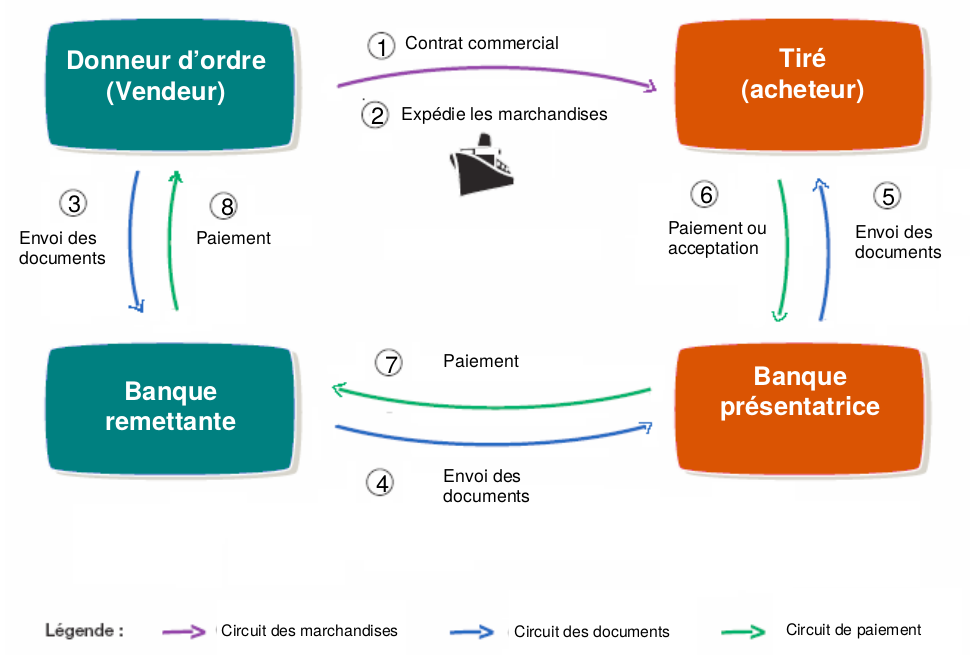
\includegraphics[width=12cm]{images/remise_doc.png}
         \caption{Circuit d'une opération de remise documentaire.
         \label{fig:remise}}
    \end{center}
   \end{figure}
   
   
 \subsubsection{Les remises de chèques hors UEMOA}
 
  La remise de chèques correspond au dépôt d'un ou de plusieurs chèques par un 
  client auprès de sa banque afin que celle-ci en assure le recouvrement. Chaque
  chèque remis doit être signé au dos par le client bénéficiaire à qui, la 
  banque demande, le plus souvent, d'indiquer le numéro de compte à créditer au 
  dos du chèque.


